% Template for seminar reports
% Computer Vision Group, Visual Computing Institute, RWTH Aachen University
\documentclass[twoside,a4paper]{article}
\usepackage[utf8]{inputenc}
\usepackage{a4}
\usepackage{fancyhdr}   
%\usepackage{german}    % Uncomment this iff you're writing the report in German
\usepackage{makeidx}
\usepackage{color}
\usepackage{t1enc}		% German letters in the "\hyphenation" - command
\usepackage{latexsym}	% math symbols
\usepackage{amssymb}    % AMS symbol fonts for LaTeX.
\usepackage{graphicx}
\usepackage{pslatex}
\usepackage{ifthen}
\usepackage{booktabs}
\usepackage[T1]{fontenc}
\usepackage{pslatex}
\usepackage{psfrag}
\usepackage{subfigure}
\usepackage{url}
\usepackage{datetime}
\usepackage{xspace}
\usepackage{multirow}
\usepackage[bb=boondox]{mathalfa}
\usepackage{biblatex}
\addbibresource{abbrev.bib}
\usepackage{float}
\restylefloat{table}
\usepackage{hyperref} 
\usepackage{acronym}
\usepackage{caption}
\usepackage{subcaption}
\usepackage{todonotes}
\usepackage{chngcntr}
\counterwithin{figure}{subsection}
\usepackage[symbols,nogroupskip,record]{glossaries-extra}
% \GlsXtrLoadResources[
%  src={symbols.bib},
%  type=symbols,% put these entries in the 'symbols' glossary
% ]


\newdateformat{monthyeardate}{\monthname[\THEMONTH] \THEYEAR}

% Do not change these sizes and do not add superfluous 
% pagebreaks to increase the page count.
\setlength{\oddsidemargin}{3.6pt}
\setlength{\evensidemargin}{22.6pt}
\setlength{\textwidth}{426.8pt}
\setlength{\textheight}{654.4pt}
\setlength{\headsep}{18pt}
\setlength{\headheight}{15pt}
\setlength{\topmargin}{-41.7pt}
\setlength{\topskip}{10pt}
\setlength{\footskip}{42pt}
\setlength{\parindent}{0pt}

\makeatletter
\DeclareRobustCommand\onedot{\futurelet\@let@token\@onedot}
\def\@onedot{\ifx\@let@token.\else.\null\fi\xspace}
\def\eg{\emph{e.g}\onedot} \def\Eg{\emph{E.g}\onedot}
\def\ie{\emph{i.e}\onedot} \def\Ie{\emph{I.e}\onedot}
\def\cf{\emph{c.f}\onedot} \def\Cf{\emph{C.f}\onedot}
\def\etc{\emph{etc}\onedot} \def\vs{\emph{vs}\onedot}
\def\wrt{w.r.t\onedot} \def\dof{d.o.f\onedot}
\def\etal{\emph{et al}\onedot}
\makeatother

% =========================================================================
\graphicspath{{pictures/}}
\setcounter{secnumdepth}{3}
\setcounter{tocdepth}{3}

% =========================================================================
\begin{document}
\pagenumbering{Roman}
\begin{titlepage}
\begin{center}
\ 
\vspace{3.5cm}

\textsf{
RWTH Aachen University \\
Faculty of Mathematics, Computer Science and Natural Sciences\\
Media Informatics
}

\rule{\linewidth}{1pt}

\vspace{1.75cm}
\LARGE
\textbf{Master's Thesis}

\vspace{1.7cm}
\huge
Development of a Source Library for Transfer Learning: Leveraging Clustering and Contrastive Learning Techniques

\vspace{3.0cm}
\Large
Sneha Banerjee\\
\large
Matriculation Number: 430069

\vspace{0.5cm}
\today

\vspace{1.05cm}
\rule{\linewidth}{1pt}

\vspace{0.5cm}
\textsf{\textbf{
\normalsize
\begin{tabular}{ll}
Examiner: & Prof. Dr. Christian Bauckhage\\
Supervisor:  & Daniel Schiller\\
\end{tabular}
}}
\end{center}

\end{titlepage}


\begin{titlepage}

\Large\textbf{Declaration of Originality}
\paragraph{}
\hskip-0.8cm
    \begin{tabular}{p{1.8in}p{4.8in}}
        Name & Sneha Banerjee \\
        Matriculation number & 430069 \\
        Address & Allmandring 8A,70569 Stuttgart \\        
        Title & \textit{Development of a Source Library for Transfer Learning: Leveraging Clustering and Contrastive Learning Techniques} \\
    \end{tabular}

\vspace{1cm}
I now declare,
\begin{itemize}
    \item that I wrote this work independently,
    \item that no sources other than those stated are used and that all statements taken from
other works—directly or figuratively—are marked as such,
    \item that the work submitted was not the subject of any other examination procedure,
either in its entirety or in substantial parts,
    \item that I have not published the work in whole or in part, and
    \item that my work does not violate any rights of third parties and that I exempt the
University against any claims of third parties.
    \end{itemize} 
\end{titlepage}
\begin{abstract}
% +++++++++++++++++++++++++
% Insert your Abstract here (one paragraph summary)
 
% +++++++++++++++++++++++++
\end{abstract}

\tableofcontents
% =========================================================================

% +++++++++++++++++++++++++
% Insert your Text here
% +++++++++++++++++++++++++

\section{Introduction}
\pagenumbering{arabic}
\subsection{Motivation}
\subsection{Task and Goal}
\subsection{Approach}
\subsection{Contribution}


\section{Related Work}

\section{Fundamentals}
\subsection{Bin Picking}
\subsubsection{Definition and Application}
\subsubsection{Gripper Types}
\subsubsection{Model-Based Approaches}
\subsubsection{Model-Free Approaches}
\subsubsection{Robot System}
\subsection{Deep learning-based 3D Image processing}
\subsubsection{Convolution Neural Network}
Inspired from the visual cortex of humans, convolutional neural network(\ac{CNN} or ConvNet) is a type of deep neural network designed for processing data which appear in a grid like manner like images, videos, etc.  It was introduced by Yann LeCun et. al in \cite{lecun1998gradient} in 1998.  It gets it name because of the usage of a special kind of linear mathematical operation called the convolution instead of using matrix multiplication as prevalent in the pre-existing neural networks. The key components of a \ac{CNN} are - Convolution layer, activation function, pooling layer, loss function, output layer. The principle building block if a CNN is the convolution layer. It consists of a number of learnable filters (kernels) which can be visualised like a cubic block. The success of \ac{CNN}s can be attributed to three major concepts: sparse interactions, parameter sharing and equivariant representations.
\paragraph{Sparse interactions}
In traditional fully connected network, matrix multiplication is performed which involves a parameter matrix. The interaction between input and output units are captured by a distinct parameter in the parameter matrix. But \ac{CNN}s have sparse interactions, i.e. only a subset of units or neurons in a layer is connected to a local region in the preceding layer. This is done by using kernels that are significantly smaller than the input. This implies, less number of parameters need to be stored which reduces the memory consumption and also it is computationally efficient because it has to perform fewer operations. For example, if there are m inputs and n outputs, the fully connected network would need to store \textit{m} x \textit{n} parameters and have a runtime of \textit{O}(\textit{m} x \textit{n}) time complexity per input. On the other hand, if we restrict the number of connections for each unit to be k, then we would have \textit{k} x \textit{n} and have a runtime of \textit{O}(\textit{k} x \textit{n}) time complexity per input, where k is quite some fold lesser in magnitude as compared to m. Moreover, since convolution layers are stacked upon one another in a deep convolution network, units in the deeper layers have a larger receptive field, because of it's indirect interaction with a larger region in the input.
\paragraph{Parameter sharing}
Another important focus behind using the convolution layer was to reduce the number of parameters in a \ac{FCN}. For example in a 1024*1024 image, a \ac{FCN} would have over 1 million hidden units, which means it would have over 1 trillion trainable parameters. But the pixels in an image are only locally correlated. So, \ac{CNN}s make use of the kernels to limit the focus on smaller regions on the image at a time known as the receptive field. This significantly reduces the number of trainable parameters, thus reducing the memory consumption. \cite{ConvNet}.    These layers perform a convolution operation between the input (eg. image) \textit{I} and the kernel \textit{K} to produce an output \textit{S} known as the feature map as in Eq.\ref{eq:conv}.
\paragraph{Equivariant Representations} 
A function is said to be equivariant if the input to a function is changed, then the output changes in the similar way. Because of the parameter sharing mechanism, convolutions operations are translation equivariant. When the kernels the applied on an input image, the convolution layers generate a 2D map of where the particular feature occurs in the particular image. Furthermore, a pixel is related to it's neighboring pixels to form a meaningful context(create a feature e.g. an edge in an image) but it is not limited to where it can occur throughout the image. Thus it creates multiple filters each of which look for the same feature throughout the image. But it is also to be kept in mind that convolution is not equivariant to other geometric and affine transformations like rotation, scaling, etc. 
 Since convolution operations are commutative in nature, Eq. \ref{eq:conv} can also be written as Eq.\ref{eq:conv_com}. Typically, Eq. \ref{eq:conv_com} is easier to incorporate into a machine learning library since values for both 'm' and 'n' varies within a small range.\cite{Goodfellow-et-al-2016}
\begin{equation}
    \label{eq:conv}
    \mathit{S(i,j)}= \mathit{(I*K)(i,j)} = \sum_{m}\sum_{n}\mathit{I(m,n)K(i-m,j-n)}
\end{equation}
\begin{equation}
    \label{eq:conv_com}
    \mathit{S(i,j)}= \mathit{(I*K)(i,j)} = \sum_{m}\sum_{n}\mathit{I(i-m,j-n)K(m,n)}
\end{equation}
\paragraph{Activation function}
The next step in a \ac{CNN} is to apply an activation function. the purpose of using a non linear activation function is to capture the non-linearity in the data. Moreover if non-linearity is not used in between the multiple layers of a neural network, the network is effectively only one layer deep which is not capable even to capture the non-linearity in real world datasets. \ac{ReLU} is the most commonly used non-linear activation function used in \ac{CNN}s because unlike sigmoid function or tanh function it does not penalise "too correct" data points. Another remarkable benefit of using \ac{ReLU} is it's ability to propagate gradient through deep networks with a constant factor. Also it is more memory efficient to use \ac{ReLU} as it doesn't require to store the \ac{ReLU} outputs separately as compared to tanh outputs.
\paragraph{Pooling}
The third step of a \ac{CNN} is to use the pooling layer. The main purpose of this operation is to make the detection of the features robust to the exact location of the eye (i.e. invariant to small translations). The different types of pooling operations are - max pooling and average pooling. It also helps in reducing the dimensionality of the input without losing too much information. This is done to make the computations faster down the deeper layers of the network. If the pooling operations are performed after every k pixels, then the next layer processes inputs that are k times lesser. Since the number of parameters in a layer are dependent on the size of the input to the layer, it significantly reduces the computational overhead on using pooling operations.
\todo{Complete CNN} 

\subsubsection{Autoencoders}
\begin{figure}
  \centering
  \begin{minipage}[t]{.45\textwidth}
    \centering
    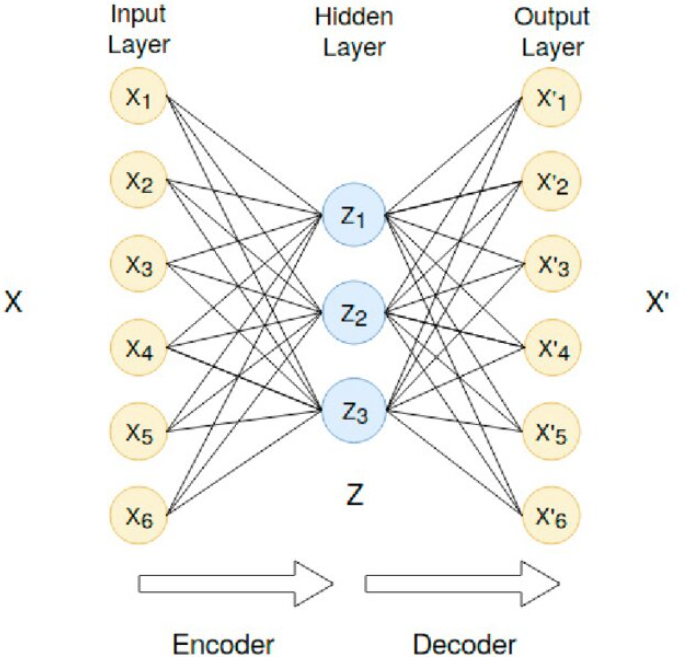
\includegraphics[width=200pt,height=150pt]{pictures/undercomplete_autoencoder.png}
    \captionof{figure}{Architecture of an undercomplete autoencoder.\cite{undercompleteautoencoder}}
    \label{fig:undercompleteautoencoder}
  \end{minipage}%
  \hspace{1cm}
  \begin{minipage}[t]{.45\textwidth}
    \centering
    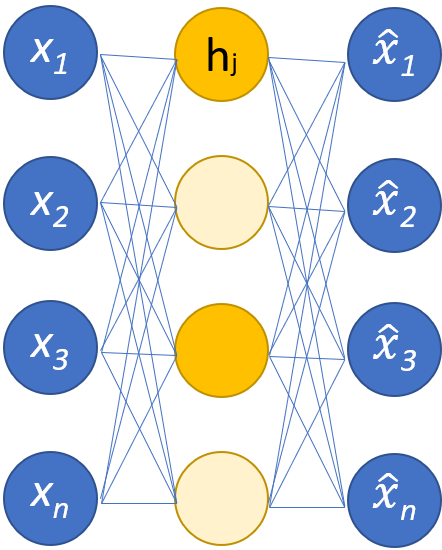
\includegraphics[width=200pt,height=150pt]{pictures/sparse_autoencoder.png}
    \captionof{figure}{Architecture of a single layer sparse encoder. The hidden nodes in bright yellow are active, while the ones in light yellow are set to zero, hence inactive\cite{autoencoder}}
    \label{fig:sparse_autoencoder}
  \end{minipage}
\end{figure}
Autoencoders are a special type of feedforward neural network in which the output tries to reconstruct the input. It is predominantly used in unsupervised learning for the tasks if dimensionality reduction, learning feature representations, and for data compression.It tries the encode the input data into a more compact representation with lower dimensions called the "code"\cite*{Goodfellow-et-al-2016} or "latent space". The idea is that this latent space representation should capture the most vital aspects pf the input data. This is done by the first part of the network called the encoder. The second part of the network, the decoder then tries to decode this compressed representation of the input data to reconstruct the original input data as accurately as possible. during the training of an autoencoder, the goal is to minimise this reconstruction loss, i.e. the difference between the original input data and the output of the decoder. There are different types of autoencoders - undercomplete autoencoders, convolutional autoencoders, regularized autoencoders, and variational autoencoders,

\vspace{5mm}


Undercomplete autoencoders ensures that the dimension of the latent space representation is less than the dimension of the original input data as show in Fig.\ref*{fig:undercompleteautoencoder}. Because, the output of the decoder to be the exact copy of the input is of no use. Rather, if the dimension of the code is less than that of the input, then it ensures that the autoencoder learns those representative features of the input data which are most salient\cite*{Goodfellow-et-al-2016}. Convolutional autoencoders are an extension of traditional autoencoders where convolution layers are used as building blocks in both the encoder and the decoder part of the autoencoder. After training the network, the encoder part is used for ectracting the features of the data and the decoder part is used for the reconstruction of the input data.

\vspace{5mm}

\begin{figure}[t]
  \centering
  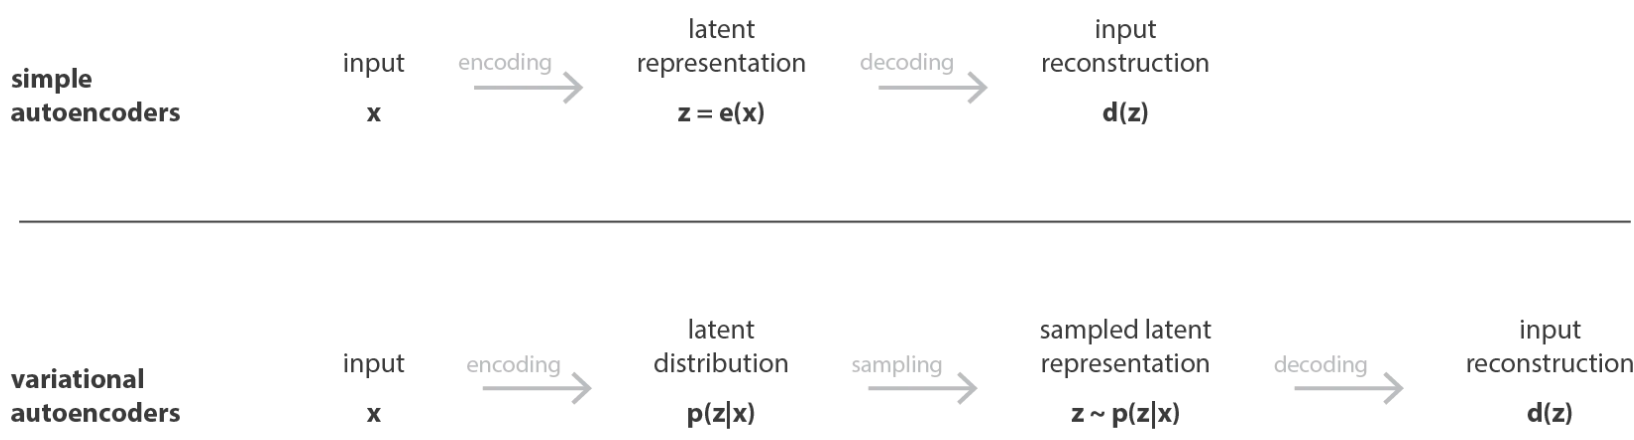
\includegraphics[width=400pt,height=150pt]{pictures/vae.png}
  \caption{Difference between a vanilla autoencoder and a \ac{VAE}.\cite{vae_image}}
  \label{fig:vae}
\end{figure} 
Regularized autoencoders are a special type of autoencoders that employs one or more regularisation techniques to prevent the model from overfitting. The different types of regularisations used are - L1 or L2 Regularisation which adds a penalty to the loss function depending on L1 or L2 norm of the model weights As a result of this, the model is capable of learning sparse representation of the training data where many weights are set to a very small value or zero as shown in Fig\ref*{fig:sparse_autoencoder}. Dropout is also used as a regularization technique where a percentage of the model's nodes are set to zero during training so that the model doesn't rely heavily on any the weight of any particular node, thus preventing overfitting and improving generalisation on unseen data. The previously mentioned regularisation techniques give rise to a variation of regularised autoencoders called the sparse autpencoders\cite*{ng2011sparse}. Sometimes noise is also added to the training data or the hidden layers of the model to increase the robustness the model giving rise to denoising autoencoders\cite*{vincent2008extracting}. One more regularisation technique if to apply a contractive regularization term based on Frobenius norm of the Jacobian matrix of the model's hidden layer activations with respect to the input data\cite*{rifai2011contractive,autoencoder}. This ensures that a small neighborhood of the input data corresponds to a small neighborhood in the latent space representation, which means small perturbations in the input data leads to small or zero variation in the latent space representation\cite*{rifai2011contractive,autoencoder}. By doing so, it makes the model more robust to small changes in the input data, thus preventing overfitting.

\vspace{5mm}

\ac{VAE}s are a distinct type of autoencoders which produces latent space representations that are continuous, which allows random sampling and interpolation for the generation of new datapoints. The difference between a vanilla autoencoder and a \ac*{VAE} is shown in Fig.\ref*{fig:vae}. Instead of producing a single vector for the latent space representation, it generates two vectors: a vector of means $\mu$ and a vector of standard deviations $\gamma$ for all datapoints. An encoding is then sampled from a distribution with mean $\mu$ and standard deviation $\gamma$. Thus even for the same input, i.e. when the mean and the standard deviation are the same, the sampled encoding would vary because of the involvement of the sampling procedure. The mean vector controls the position where the encoding of the input should have it's centre and the standard deviation controls the area over which the sampled encoding is allowed to vary from the mean. As a result of this, the decoder learns to decode not just the encoding of a single point but also the points in the neighborhood and hence a continuous latent space representation is obtained. In order to ensure that the latent space representation satisfies that the nearby encoding are similar to each other on a local scale while also facilitating interpolation on a global scale \ac{VAE}s jointly optimizes the reconstruction loss and the \ac*{KL}\cite*{kullback1951information} loss.\cite*{kingma2019introduction,vae}

\subsubsection{PointNet Autoencoder}
\subsubsection{Siamese Network}
\begin{figure}
  \centering
  \begin{minipage}[t]{.45\textwidth}
    \centering
    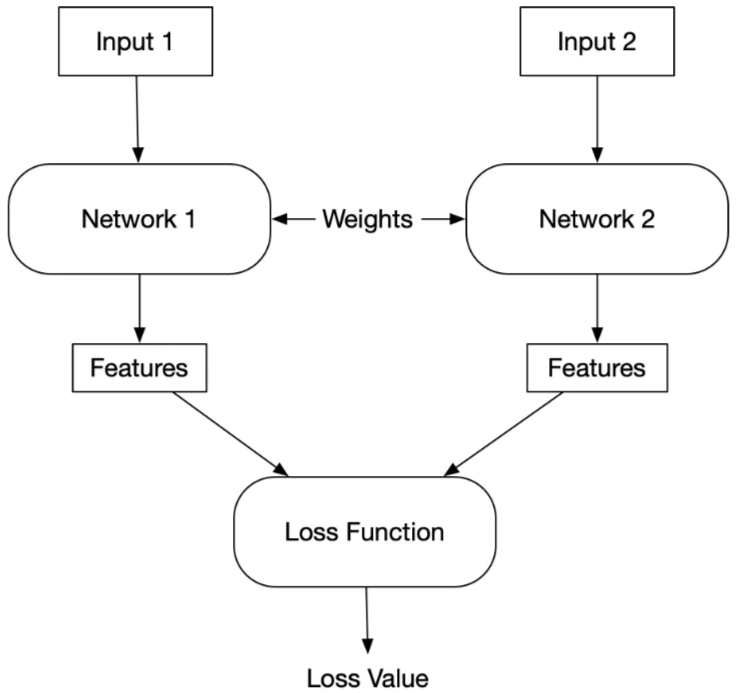
\includegraphics[width=200pt,height=120pt]{pictures/siamese_network.png}
    \captionof{figure}{A generic siamese network.\cite{siamese_network}}
    \label{fig:siamese_network}
  \end{minipage}%
  \hspace{1cm}
  \begin{minipage}[t]{.45\textwidth}
    \centering
    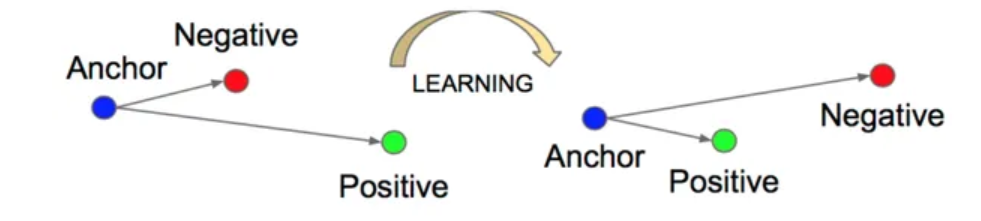
\includegraphics[width=200pt,height=100pt]{pictures/triplet_loss.PNG}
    \captionof{figure}{Before (left) and after (right) minimizing triplet loss function\cite{triplet_loss}}
    \label{fig:triplet_loss}
  \end{minipage}
\end{figure}
Traditional deep learning models have shown ground breaking results in a multitude of applications like image recognition and classification, web scraping, speech recognition and caption generation. But it has a limitation that the models tend to perform well if the training and testing data points are from the same distribution. If the model is to be made capable to predict datapoints belonging to an unknown class, we need to re-train the model with an abundant number of training samples from that class and then predict it with unseen samples of that class. This technique can often be computationally expensive and can increase expotentially if the number of classes increases. Also generating a huge number of samples for a new class of objects can be tedious and quite challenging in multiple scenarios. The Siamese network\cite*{koch2015siamese,bromley1993signature} is one such way to mitigate the above mentioned problem. The idea behind siamese networks is that two identical copies of the neural neural network with shared weights process two distinct datapoints as shown in Fig.\ref*{fig:siamese_network}. Because the networks have shared parameters, it ensures that two very similar datapoints cannot have too different locations in the feature maps as both the networks evaluate the same function. In siamese networks, the model learns a similarity function, the loss function, which plays the pivotal role in determining how similar or dissimilarthe datapoints are to one another. The two main loss functions used in siamese networks are contrastive loss function\cite*{bromley1993signature} and triplet loss function\cite*{balntas2016learning}. Since the goal of a siamese network is not to perform classification task on datapoints, rather to compute the similarity between them, contrative loss functions are more suited for this task as compared to cross-entropy loss functions, as it is for classification tasks.

\vspace{5mm}

\textbf{Contrastive loss} function evaluates how capable a siamese network is in deciding the similarity between two given datapoints as is given by Eq.\ref*{eq:contrastive_loss}\cite*{siamese_network}

\begin{equation}
  \label{eq:contrastive_loss}
  \mathcal{L}_{\textrm{con}}(Y,D_{w})= (1-Y)\frac{1}{2}(D_{w})^2 + (Y)\frac{1}{2}{max(0,m-D_{w})}^2
\end{equation}
where $\mathcal{L}_{\textrm{con}}$ is the calculated contrastive loss, $D_{w}$ is the Euclidean distance between the outputs of the twin networks\cite*{siamese_network}. Y takes the value 0 or 1. If the two datapoints belong to the same class then Y takes the value 0, otherwise it takes the value 1\cite*{siamese_network}. max() is a function to choose the higher of the two values, 0 or $m-D_{w}$ where m is the margin and has a value greater than 0\cite*{siamese_network}. The usage of a margin in this equation ensures that the pair of datapoints which the dissimilar beyond this margin value are excluded while calculating the loss function\cite*{siamese_network}. The euclidean distance between the embeddings of the two datapoints are given by the Eq.\ref*{eq:euclidean_dist}\cite*{siamese_network}
\begin{equation}
  \label{eq:euclidean_dist}
  D_{w}(X_{1},X_{2})= \sqrt[2]{\{G_{w}(X_{1}) - G_{w}(X_{2})\}^2}
\end{equation}
where $G_{w}(X_{i})$ is the output of the twin network such that $i \in \{1,2\}$ as show in Fig.\ref*{fig:siamese_network}.
\begin{figure}
  \centering
  \begin{minipage}[t]{.45\textwidth}
    \centering
    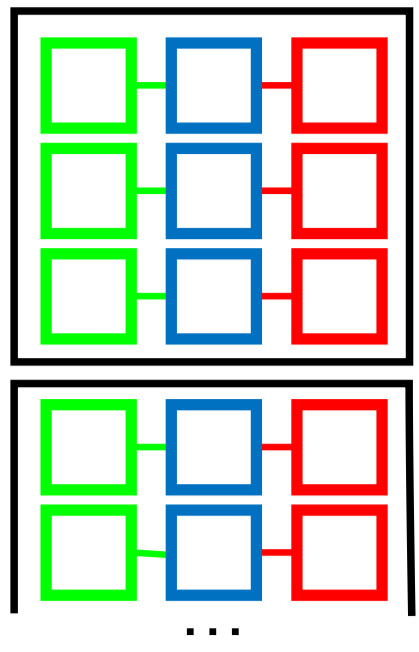
\includegraphics[width=100pt,height=120pt]{pictures/offline_triplet.jpg}
    \captionof{figure}{Minibatches in offline triplet mining. The green boxes are positive datapoints, the blue boxes are anchor datapoints and the red boxes are negative datapoints.}
    \label{fig:offline_triplet}
  \end{minipage}%
  \hspace{1cm}
  \begin{minipage}[t]{.45\textwidth}
    \centering
    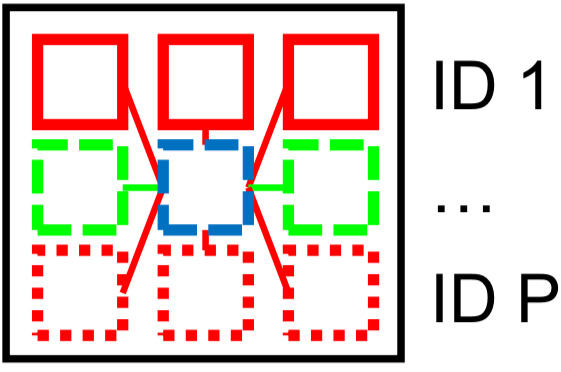
\includegraphics[width=100pt,height=120pt]{pictures/online_triplet.jpg}
    \captionof{figure}{Triplets constructed only within the minibatch. There are P object classes in the minibatch. The green boxes are positive datapoints, the blue boxe is the anchor datapoint and the red boxes are negative datapoints.}
    \label{fig:online_triplet}
  \end{minipage}
\end{figure}
\textbf{Triplet loss} function\cite*{weinberger2009distance} trains the siamese network in a way that a triplet of datapoints are presented to the siamese network. by applying triplet loss the model tries to group the datapoints similar to the anchor datapoint, close to one another while increasing the distance between the anchor datapoint and the datapoints dissimilar to it as shown in Fig.\ref*{fig:triplet_loss}. In order to do so, a positive value called margin is used which increases the distance between dissimilar datapoints and also eliminates the output of any trivial solution. Euclidean distance or cosine distance is used as the distance metric while calculating the triplet loss and shown in Eq.\ref*{eq:triplet_loss}\cite*{hermans2017defense,siamese_network}
\begin{equation}
  \label{eq:triplet_loss}
  \mathcal{L}_{\textrm{tri}}(a,p,n)=\sum_{\substack{a,p,n \\ y_{a}=y_{p}!=y_{n}}} max(0,d(a,p)-d(a,n)+margin)
\end{equation}
where $y_{x}$ is the class label for the datapoint x for $x \in \{a,p,n\}$, a is the anchor datapoint, p is the positive example having the same class label as the anchor datapoint and n is the negative example having a different class label as compared to the anchor datapoint.
but there are some practical problems related to the use of triplet loss function. The number of possible triplets grow cubically with the increase in the size of the dataset. Also most of the triplets are often uninformative. Thus mining "hard triplets" or the ones crucial for the learning of the model becomes a challenging task. As per the definition of the triplet loss function, the triplets can be of three types: easy triplets, hard triplets and medium hard triplets. The triplets which satisfy the condition $d(a,p)+margin<d(a,n)$ results to the loss value being 0, hence are called the easy triplets.\cite*{triplet_loss} For the triplet for which the negative datapoint is closer to the anchor as compared to the positive datapoint i.e. $d(a,n)<d(a,p)$ are the examples of hard triplets.\cite*{triplet_loss} And the medium hard triplets are the ones where the negative datapoints are not closer to the anchor datapoint as compared to the positive datapoint but still results in positive loss i.e. $d(a,p)<d(a,n)<d(a,p)+margin$.\cite*{triplet_loss} Thus the medium hard triplets are the most essential for the model training as they constitute for the most useful information. Two triplet mining procedures are used to mitigate the issue of excessive computational overhead with increase in dataset size. They are offline triplet mining and online triplet mining. In offline hard triplet mining, at first the dataset is manually processed to find hard triplets and then they are used for training the model. But manually finding the hard triplets can be quite tedious. Online triplet mining is a better approach as compared to the one mentioned above. The model is trained in minibatches of the dataset as shown in Fig.\ref*{fig:offline_triplet}. Using only the triplets that were mined from the dataset could be a wasteful design choice in such scenario. So in a minibatch, it containes way more potential triplets than the ones that were mined. So each member of another triplet becomes an additional negative datapoint example. But both hard positive and hard negative datapoints are required for training. An even better design to mitigate that would be to choose let's say K datapoints from P different classes in the dataset, where the K positive examples serve as hard positives while the rest of the datapoints in the minibatch serve as hard negatives as shown in Fig.\ref*{fig:online_triplet}\cite*{hermans2017defense}.

\vspace{5mm}

Thus siamese networks are very robust to the class imbalance in dataset which is very common in real datasets. Since it depends on very few datapoints of a particular object class, it has good generalisation capabilities for unseen datapoints in the future. They are also very robust to small perturbationsin the datapoints due to difference in lighting conditions or orientation or background, as they keep similar objects close to each other even if the datapoints are slightly different. Since the siamese networks places similar datapoints together while increasing the distance between dissimilar datapoints, they are often useful for learning semantic similarity within the datapoints. However despite it's benefit, training a siamese network takes longer as compared to traditional neural networks because it involves learning from quadratic pair of datapoints.\cite*{siamese_network}
\subsection{Clustering Algorithms}
\begin{figure}[t]
  \centering
  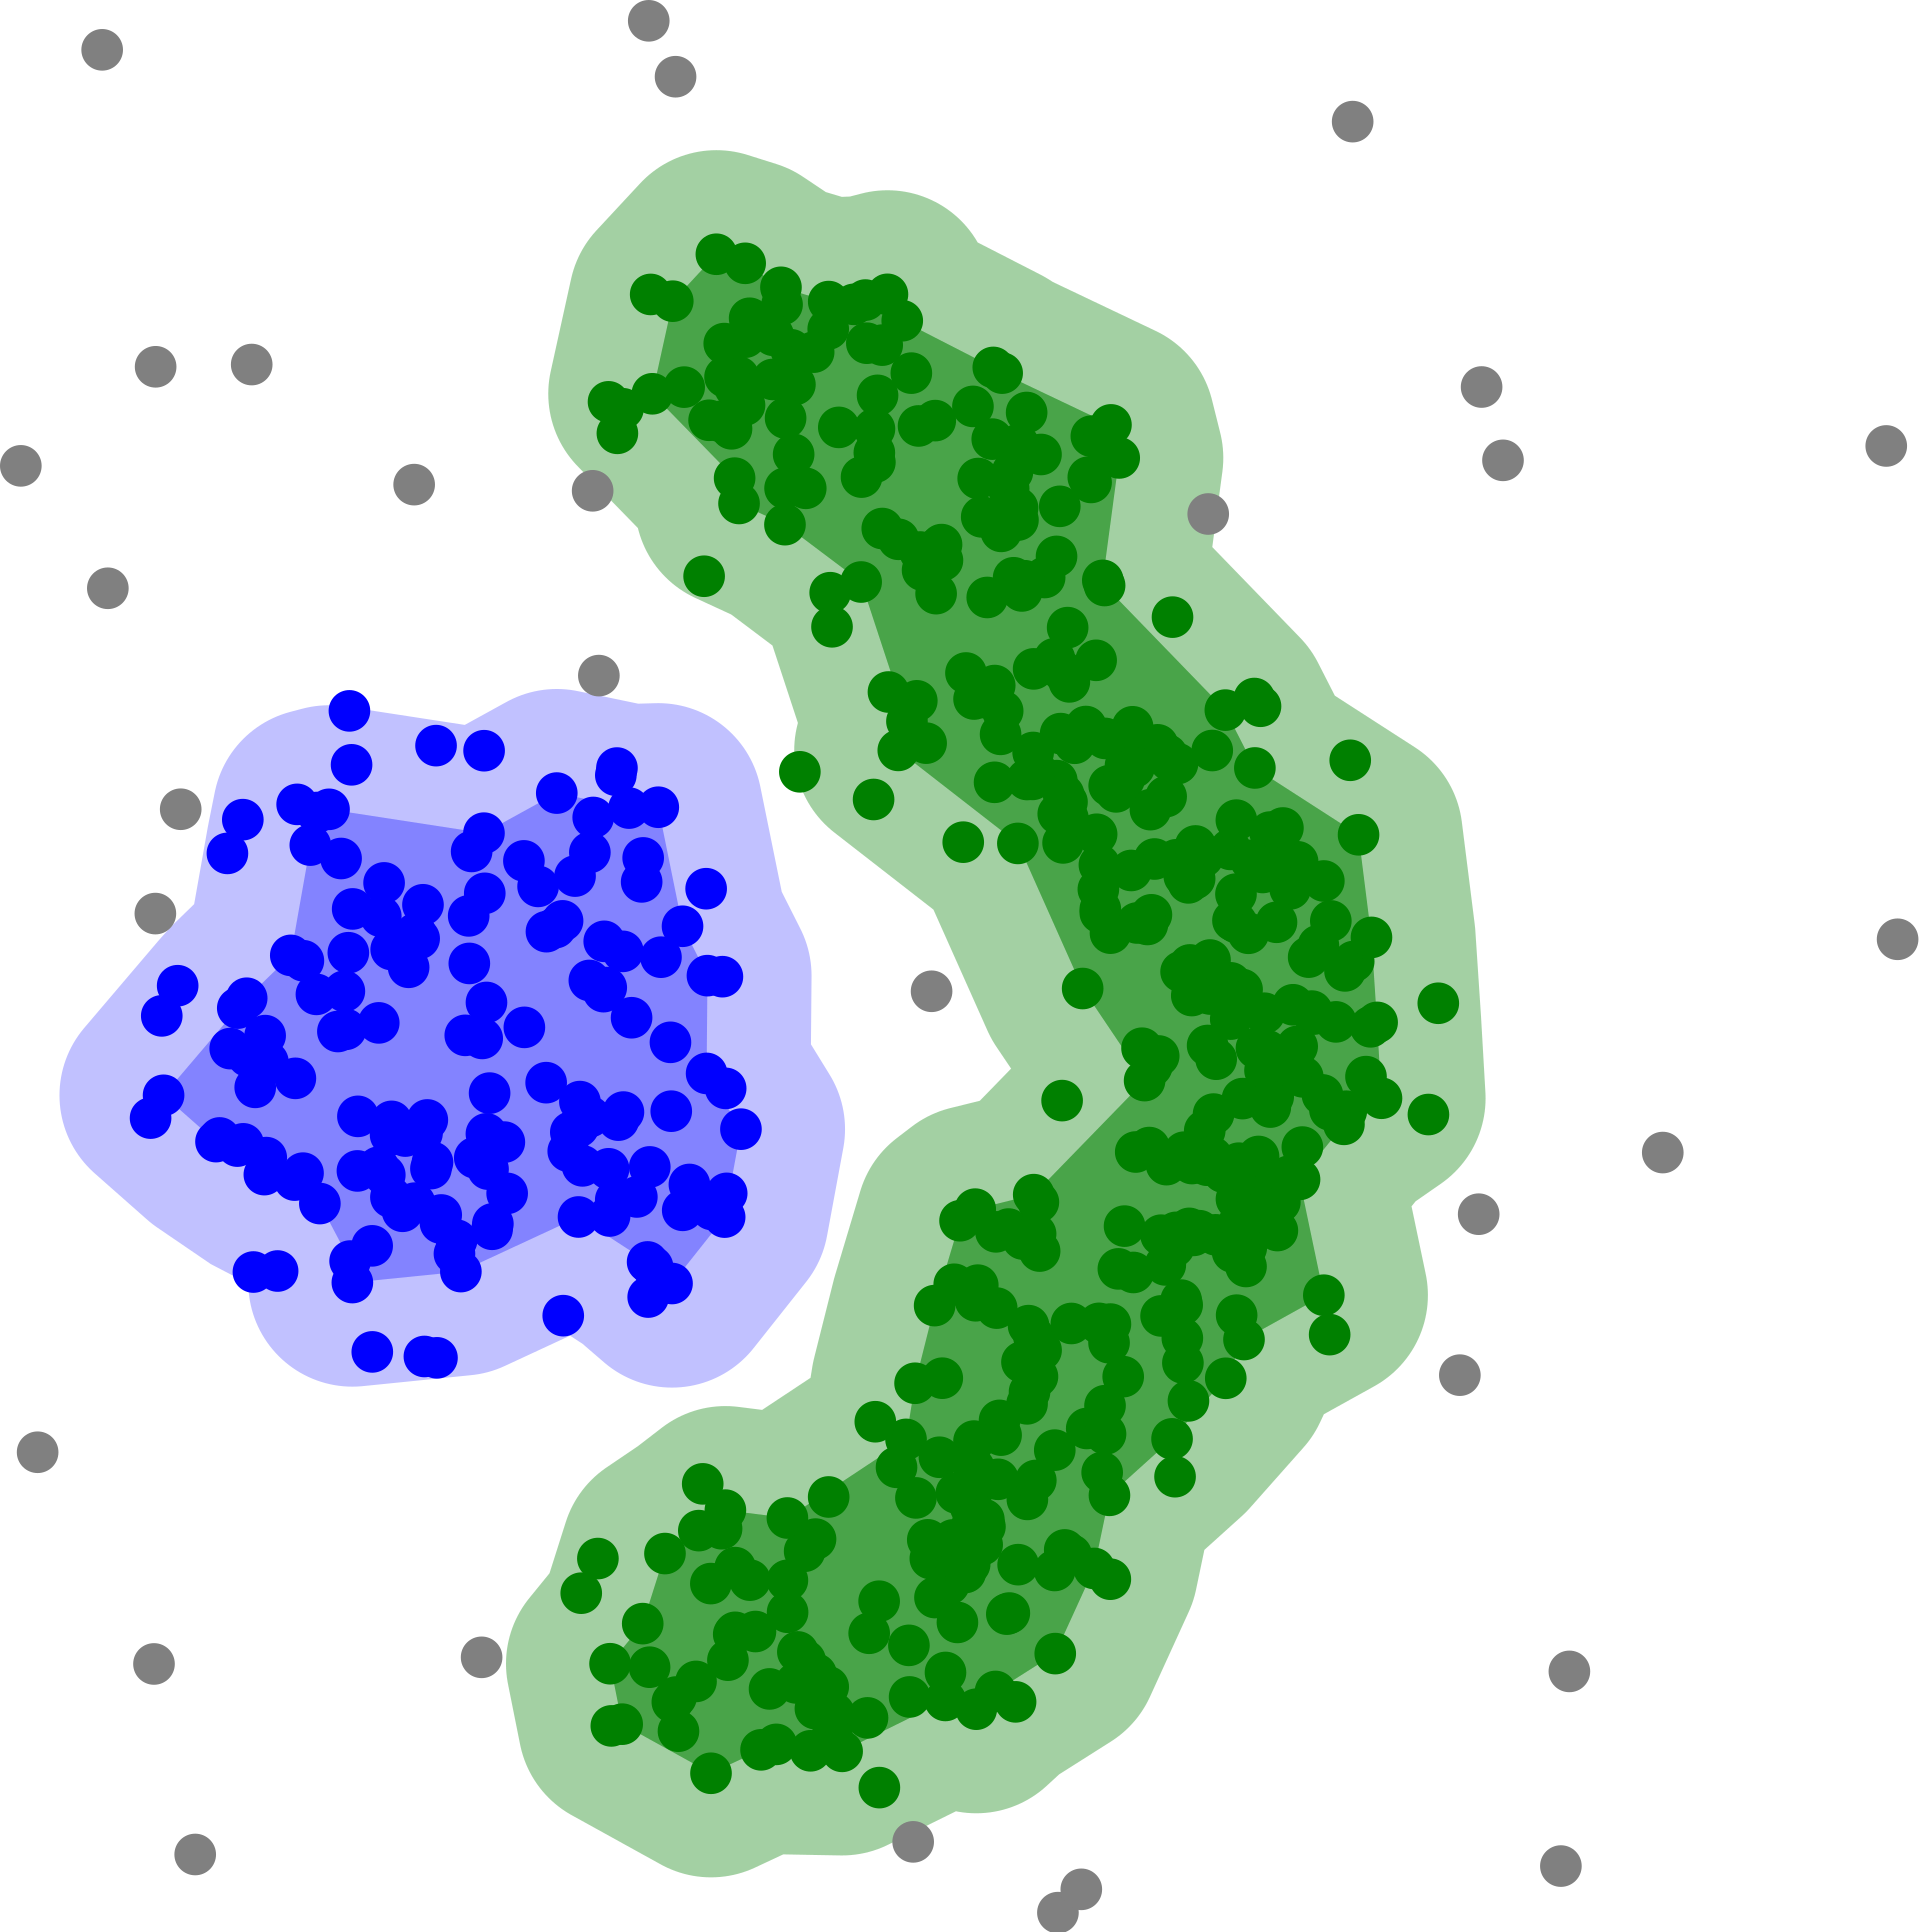
\includegraphics[width=200pt,height=150pt]{pictures/DBSCAN-density-data.png}
  \caption{\ac{DBSCAN} can find non-linearly separable non-convex clusters.\cite{dbscanWiki}}
  \label{fig:dbscan}
\end{figure} 
When the dataset does not have any labelled data, then it is said to be unsupervised learning. In this case, there is no ground truth available to measure the correctness of the outputs generated by the \ac{ML} models. The primary focus of unsupervised learning is to find hidden and interesting pattern in the data. Unsupervised learning is of utmost importance in the \ac{AI} world as several real world datasets do not have available annotations, which requires a lot of human effort. Unsupervised learning algortihms can be broadly categorized into the following domains-clustering, dimensionality reduction, and association analysis. Clustering algorithms aim at grouping unlabelled data into groups or clusters based on how similar or dissimilar the datapoints are to one another. It can reveil underlaying hidden pattern in the data and is used in applications like image segmentation, fraud detection, etc. Dimensionality reduction is reduces the number of irrelavant features or dimensions of the dataset. The inclusion of more features does help in the better representation of the dataset but it also significantly increases the memory consumption and complexity to work with it. Also it is often difficult to visualise real-life datasets with too many features. Association analysisis a rule-based unsupervised learning method that reveals the relationship between attributes in the dataset. It is used in applications like market analysis, intrusion detection, etc.Clustering algorithms can be broadly classified into the following categories: density-based, distribution-based, and hierarchical-based.\\
\begin{figure}
  \centering
  \begin{minipage}[t]{.45\textwidth}
    \centering
    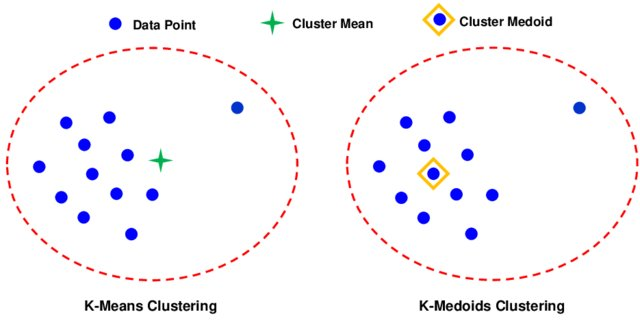
\includegraphics[width=200pt,height=150pt]{pictures/The-graphical-representation-of-the-difference-between-the-k-means-and-k-medoids_W640.jpg}
    \captionof{figure}{Difference between K-Means and K-Medoids.\cite{kmean-kmedoid}}
    \label{fig:kmean-kmedoid}
  \end{minipage}%
  \hspace{1cm}
  \begin{minipage}[t]{.45\textwidth}
    \centering
    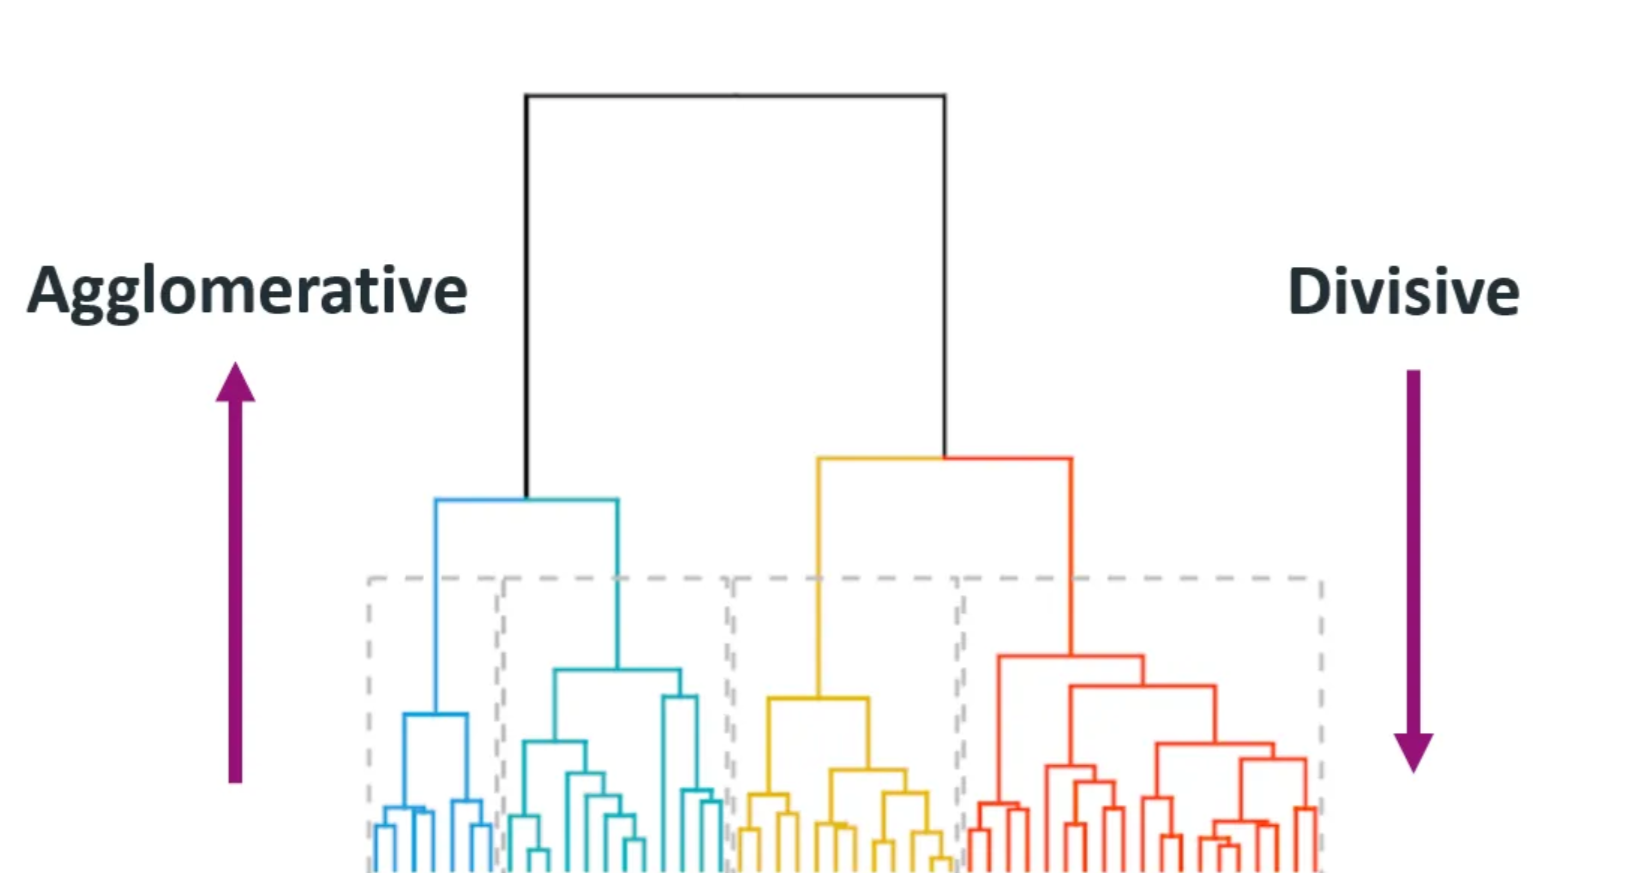
\includegraphics[width=200pt,height=150pt]{pictures/dendogram.png}
    \captionof{figure}{A dendogram in hierarchical clustering.\cite{dendogram}}
    \label{fig:dendogram}
  \end{minipage}
\end{figure}
\subsubsection{Density-based Clustering}
 In density-based clustering, the algorithm looks for areas of high concentration of the datapoints and groups them as a cluster. The benefit of this algorithm is that the shape a cluster can be is not limited and hence doesn't necessarily have to be convex in nature as show in Fig. \ref*{fig:dbscan}.
Moreover, these algorithms are also very robust to outliers as they do not force the outliers to belong to any category but are rather ignored as it is unlikely that outliers can form an area of high concentration of datapoints. I have carried on the experiments on this thesis on two such density-based clustering algortihms called \ac{DBSCAN}\cite*{dbscan} and \ac{HDBSCAN} algorithms\cite*{hdbscan}. The available scikit-learn implementations were used for this purpose\cite*{scikit-learn}. The \ac{DBSCAN}\cite*{dbscan} algortihm  does not require the users to define the number of clusters to be generated which doesn't force dissimilar datapoints to belong to the same cluster. However, this algorithm was still sensitive to two parameters $\epsilon$, the maximum distance betwwen the datapoints to be considered in the same cluster and the minimum number of samples in the cluster which the user needs to define \cite*{scikit-learn}. But finding an optimum value for these parameters often require domain expertise and are dependent on the data. The \ac{HDBSCAN}\cite*{hdbscan} algorithm mitigates this issue and thus does not require the user to define these two parameters. It is a hierarchical density-based clustering that performs the \ac{DBSCAN} algorithm over multiple $\epsilon$ values to find the most stable result. 

\subsubsection{Distribution-based Clustering}
In distribution-based algorithms, a datapoint is said to be a member of the cluster depending on the probability of it's membership to the cluster. The more the distance of a point increases from the centre of the cluster, the less is it's probability of belonging to that cluster. Centroid-based algorithms groups the datapoints based on some initial cluster centres. Once all the dataspoints are softly assigned to some cluster membership, the cluster centres are recalculated and this process is iterated until convergence. These algorithms are sensitive to the initial parameters like the cluster centres chosen in the first step. Another major disadvantage of these clustering algorithms are that they always form spherical clusters. The user also needs to define the number of clusters the dataset is to be grouped in, which makes it sensitive to outliers. However, these algorithms can be executed very fast and we have used two such algorithms in our experiments- K-Means\cite*{kmeans}and K-Medoids\cite*{kmedoids}. In K-Means, the mean of the datapoints of the clusters is assigned as the cluster-centroid. It might not be an actual datapoint in the dataset, rather a blurred, noisy average of a datapoints in the cluster. On the contrary, the K-Medoids algortihm assigns an actual datapoint of the dataset, that is most centrally located as the cluster centroid as shown in Fig.\ref*{fig:kmean-kmedoid}. Thus K-Medoids is more robust to outliers and noises as compared to K-Means.

\subsubsection{Hierarchical-based Clustering}
Hierarchical-based clustering algorithm that form a hierarchy of clusters. Datapoints in a cluster are more similar to each other as compared to other groups. this hierarchy of clusters is visualised by a hierarchy tree called dendograms. hierarchical clustering algorithms can be of two types - agglomerative and divisive. In agglomerative clustering, each datapoint is considered as a separate cluster in the first step. Then these clusters are merged into one another until only one cluster remains. Thus at the end, the last level cluster consists of all teh datapoints in the dataset. The divisive method is the reverse procedure of the aggomerative method. In the beginning, all the datapoints are considered to be in a single cluster and gradually the cluster is broken into smaller clusters, untill each cluster consists of only one datapoint. A visual representation of a dendogram has been shown in Fig.\ref*{fig:dendogram}
\subsection{Evaluation metrics for Clustering Algorithms}
The ground truth or labels are available in supervised learning. So to determine the quality of the clustering algorithm we can calculate the level of accuracy by comparing the labels predicted by a model to the ground truth. But most real world datasets do not have ground truth. Therefore, it makes it challenging in unsupervised learning paradigm to determine the quality of the clustering algorithm. But a good clustering algorithm is still expected to have little difference between the objects in a cluster i.e. small within-cluster variance and more difference between objects from different clusters i.e. large between-cluster variance. Thus the evaluation metrics used in the literature could be categorised into two broad groups: extrinsic measures and intrinsic measures, depending on the availability of the ground truth. Extrinsic measures, when the ground truth is available uses metrices like Rand Index, Mutual Information, V-measure and Fowlkes-Mallows Scores. Intrinsic measures, when the ground truth is not available mostly uses Silhouette Score, Calinski Harabaz Index and David Bouldin index.

\vspace{5 mm}

\textbf{Silhouette Score} is used to calculate the distance between points within a cluster as compared to it's distance from the points in the neighbouring cluster and is given by Eq. \ref*{eq:silhouette_score}
\begin{equation}
  \label{eq:silhouette_score}
  \mathit{S_{c}}= \mathit{\frac{(n_{c}-i_{c})}{max(n_{c},i_{c})}}
\end{equation}
where $S_{c}$ is the Silhouette Coefficient, $n_{c}$ is the average of the nearest-cluster distance of each datapoint and $i_{c}$ is the average distance between the datapoint within the cluster. The Silhouette coefficient lies within the range $[-1,1]$, where the the more closer the coefficient is to 1, the better is the clustering results. When the Silhouette Coefficient is close to 0, it implies that the datapoints are on or very close to the decision boundary between adjacent clusters, whereas negative values imply that the datapoints have been wrongly classified. But the drawbacks of using this metric is that is tends to favour dense and convex clusters. Since it takes into account, the average of teh distance within a cluster as well as between adjacent clusters, it doesn't perform well different clusters have a significant difference in their respective sizes, which is quite a common phenomenon in real world datasets. The chosen distance metric for the calculation of the Silhouette score also has a significant effect on it and can lead to very different results.

\vspace{5 mm}

\textbf{Calinski-Harabasz Index}(C-H Index) or the Variance Ratio Criterion is used to measure the dispersion between the datapoints within a cluster as compared to in-between clusters as in given by Eq. \ref*{eq:c-h index}
\begin{equation}
  \label{eq:c-h index}
  \mathit{S_{CH}}= \mathit{\frac{tr(B_{k})}{tr(W_{k})}} \times \mathit{\frac{(n_{E}-k)}{k-1}}
\end{equation}
where $S_{CH}$ is the C-H Index, $tr(B_{k})$ is the trace of the in-between cluster dispersion matrix is in Eq. \ref*{eq:Bk}  and $tr(W_{k})$ is the trace of the within-cluster dispersion matrix as in Eq. \ref*{eq:Wk}
\begin{equation}
  \label{eq:Bk}
  \mathit{B_{k}}= \mathit{\sum_{q=1}^{k}n_{q}(c_{q}-c_{o})(c_{q}-c_{o})^T} 
\end{equation}
\begin{equation}
  \label{eq:Wk}
  \mathit{W_{k}}= \mathit{\sum_{q=1}^{k}\sum_{x \in C_{q}}(x-c_{q})(x-c_{q})^T} 
\end{equation}
where $c_{q}$ is the centroid of the cluster $q$ and $c_{o}$ is the overall centroid of the datapoints. $B_{k}$ calculates the quality of the separation between two clusters, i.e., higher the value of $B_{k}$, better it is. $W_{k}$ calculates the distance of a datapoint ($s$) from the centroid of the cluster, and thus measures the cohesiveness or compactness of the datapoints within a cluster, i.e, smaller the value of $W_{k}$, better it is. Distribution-based clustering algorithms like K-Means tries to minimise the value of $W_{k}$. Thus according to the equation of C-H Index in Eq. \ref*{eq:c-h index}, the higher the C-H index, the better is the clustering results. Because sum-of squared Euclidean distance is used to calculate the distance of the datapoints from their respective cluster centroids, C-H Index tends to favour convex clusters, which is a major drawback of using this metric as in Silhouette Coefficient.\cite*{chindex}
\subsection{Transfer learning}
Transfer learning is an optimization in machine learning techniques where a model trained for a particular task let's say task 1 is used for another task, task 2. It uses the knowledge learnt by the model in the previous task to be adapted for the new task. Trasnfer learning has it's benefits in a multitude of applications because real world problems doesn't necessarily always have an abundant amount of labelled data which can beused to train a model from scratch\cite*{weiss2016survey}. It can be used for tasks which intend to solve different but related problems\cite{weiss2016survey}. In other words, if the domain of the data for task 2 is similar to that of task 1, transfer learning can be used as shown in Fig.\ref*{fig:source_target}.Several approaches have been adapted to use transfer learning. Let's say we want to solve task $T_{1}$, but we don't have adequate data to train a deep neural network for it. But we have ample data to solve a similar task $T_{2}$. So we can train a model for task $T_{2}$ and then use it for task $T_{1}$. We might need to re-train only the later layers or all the layers of the model, but that heavily depends on the problem at hand. Another approach could be to use an existing pre-trained network. There are a lot a available open-source models which can be re-trained and re-used depending on the problem. Some of the popular models that are used as pre-trained models in transfer learning are Oxford VGG Model\cite*{simonyan2014very},Google Inception model\cite*{szegedy2015going}, Microsoft ResNet model\cite*{he2016deep}. Another approach could be to use transfer learning for the purpose of feature extraction. Transfer learning has found a lot of application in the domain of computer vision and natural language processing because it requires a lot of data for training such complex models from scratch. In the domain of computer vision, we know that the early layers of a deep neural network focuses on learning the low level features like the detection of edges, while the middle layers focus on learning the mid level features like the detection of shapes. In transfer learning, these pre-trained early and middle layers could be used verbatim and only the latter layers which focus on the high level features could be re-trained for the new task as shown in fig\ref*{fig:transfer_learning}.
\begin{figure}
  \centering
  \begin{minipage}[t]{.45\textwidth}
    \centering
    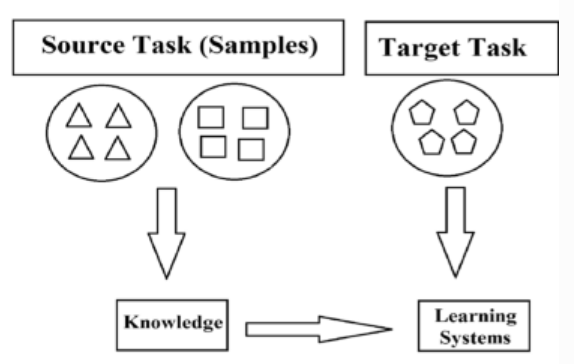
\includegraphics[width=100pt,height=120pt]{pictures/source_target.PNG}
    \captionof{figure}{Model trained for a task in the similar domain is re-used for a new task.\cite*{hosna2022transfer}}
    \label{fig:source_target}
  \end{minipage}%
  \hspace{1cm}
  \begin{minipage}[t]{.45\textwidth}
    \centering
    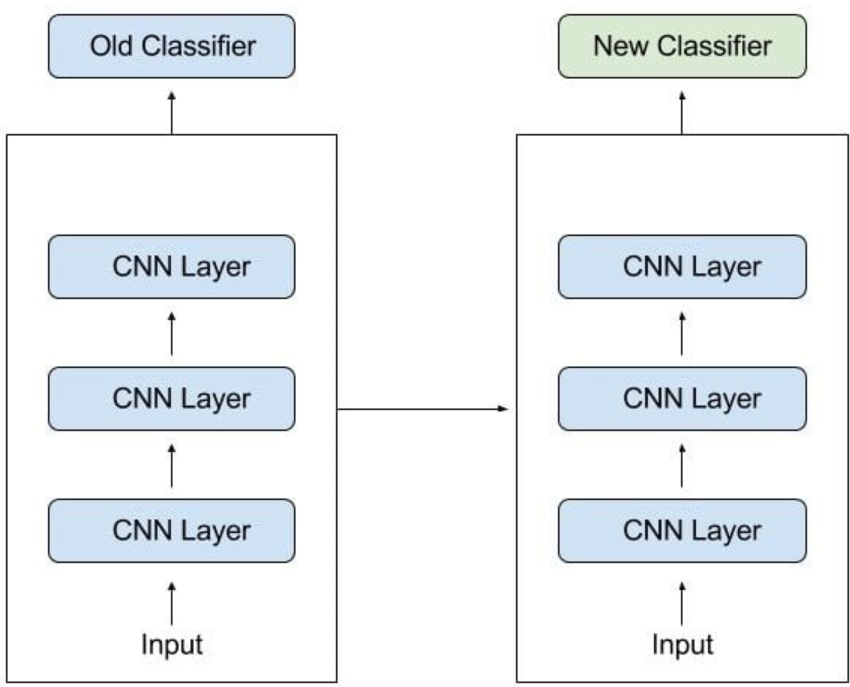
\includegraphics[width=100pt,height=120pt]{pictures/transfer_learning.PNG}
    \captionof{figure}{A model trained on a different task is adapted to be used for a new task.\cite*{transfer_learning}}
    \label{fig:transfer_learning}
  \end{minipage}  
\end{figure}
Transfer learning has numerous advantages like significant reduction in the amount of training time\cite*{liu2019exploring}, improvement in performance for some neural networks\cite*{pan2011transfer} and less reliance on a huge amount of data\cite*{duan2012learning,kulis2011you,zhu2011heterogeneous}.  
\subsubsection{Definition}
According to \cite*{weiss2016survey,pan2009survey}, transfer learning can be formally defined as the following. A domain $\mathcal{D}$ of the input data, with the feature space $\mathcal{X}$ and a marginal probability distribution $P(X)$ such that $X=\{x_{1},.....,x_{n}\} \in \mathcal{X}$, where $n$ is the number of feature vectors in $X$. In the given input data domain $\mathcal{D}$, the task $\mathcal{T}$ has a label space $\mathcal{Y}$ and a predictive function $f(\cdot)$ which is learned from the feature vector and label pairs $(x_{i},y_{i})$ such that $x_{i} \in \mathcal{X}$ and $y_{i} \in \mathcal{Y}$ and $f(x)$ is the learner that predicts the label value for x. As per the above definition, the source domain is defined as $\mathcal{D_{\mathcal{S}}}$ and the corresponding source task as $\mathcal{T_{\mathcal{S}}}$.The target domain is defined as $\mathcal{D_{\mathcal{T}}}$ and the corresponding target task as $\mathcal{T_{\mathcal{T}}}$. Transfer learning aims at improving the target predictive function $f_{\mathcal{T}}(\cdot)$ by using the related information from $\mathcal{D_{\mathcal{S}}}$ and $\mathcal{T_{\mathcal{S}}}$ where $\mathcal{D_{\mathcal{S}}}\neq \mathcal{D_{\mathcal{T}}}$ or $\mathcal{T_{\mathcal{S}}}\neq \mathcal{T_{\mathcal{T}}}$. Since $\mathcal{D_{\mathcal{S}}} = \{\mathcal{X_{\mathcal{S}}},P(X_{\mathcal{S}})\}$ and $\mathcal{D_{\mathcal{T}}} = \{\mathcal{X_{\mathcal{T}}},P(X_{\mathcal{T}})\}$, here the condition $\mathcal{D_{\mathcal{S}}}\neq \mathcal{D_{\mathcal{T}}}$ means that $\mathcal{X_{\mathcal{S}}}\neq \mathcal{X_{\mathcal{T}}}$ and/or $P(X_{\mathcal{S}}) \neq P(X_{\mathcal{T}})$.The scenario where $\mathcal{X_{\mathcal{S}}}\neq \mathcal{X_{\mathcal{T}}}$ in the context of transfer learning is defined as heterogeneous transfer learning. The scenario where $\mathcal{X_{\mathcal{S}}} = \mathcal{X_{\mathcal{T}}}$ is defined as homogeneous transfer learning. The scenario where $P(X_{\mathcal{S}}) \neq P(X_{\mathcal{T}})$ means the source and the target data are from different domains, i.e., they belong to different marginal distributions. Transfer learning algortihms are not expected to give optimal results in ths case. Refering back to the definition of transfer learning, when $\mathcal{T_{\mathcal{S}}}\neq \mathcal{T_{\mathcal{T}}}$ and it was defined that $\mathcal{T} = \{\mathcal(Y),P(Y|X)\}$. this scenario is possible when $\mathcal{Y_{\mathcal{S}}} \neq \mathcal{Y_{\mathcal{T}}}$ and/or $P(Y_{\mathcal{S}}|X_{\mathcal{S}}) \neq P(Y_{\mathcal{T}}|X_{\mathcal{T}})$. The scenario where $P(Y_{\mathcal{S}}|X_{\mathcal{S}}) \neq P(Y_{\mathcal{T}}|X_{\mathcal{T}})$ implies that the conditional probability distributions between the source and target domains are different. The case $\mathcal{Y_{\mathcal{S}}} \neq \mathcal{Y_{\mathcal{T}}}$ mean the label space of the source and target domain are different.\cite*{weiss2016survey}
\subsubsection{Categories}
As per the definition of transfer learning mentioned above, it can be broadly categorized into 3 groups: inductive transfer learning, transductive transfer learning and unsupervised transfer learning as mentioned in \cite*{pan2009survey}. Depending on the availability of labels of the source and target tasks, these 3 categories are possible as shown in Table \ref*{tab:transfer_learning}.\\
\begin{table}[t]
  \centering
  \begin{tabular}{p{1.0in}|p{1.4in}|p{1.0in}|p{1.0in}|p{0.7in}}
  \toprule
    Transfer learning Settings & Related areas & Source Domain Labels & Target Domain Labels & Tasks \\\cline{1-5}
    \multirow{2}{1.0in}{Inductive Transfer Learning} & Multi-task learning & Available & Available & \multirow{3}{0.7in}{Regression, Classification} \\\cline{2-4}
    & Self-taught Learning & Unavailable & Available \\\cline{1-4}
    Transductive Transfer Learning & Domain Adaptation, Simple Selection bias, Co-variate Shift & Available & Unavailable \\\cline{1-5}
    Unsupervised Transfer Learning &  & Unavailable & Unavailable & Clustering, Dimensionality Reduction\\  
  \bottomrule    
  \end{tabular}
  \caption{Different settings of transfer learning \cite{pan2009survey}}
  \label{tab:transfer_learning}
\end{table}
Regardless of whether the source and target domains are the same or not, the target task in an inductive transfer learning situation is distinct from the source task. In this instance, in order to generate an objective predictive function  $f_{\mathcal{T}}(\cdot)$ for usage in the target domain, some labeled data from the target domain are needed. Furthermore, inductive transfer learning can be broken down into two groups depending on the availability of source and target domain labels. When a lot of labeled data is available for the source domain, it is similar to multi-task learning. But the difference lies in the fact that the goal of inductive transfer learning is to attain good results inthe target task only by using the knowledge obtained from the source task while multi-task learning endeavors to learn both the target and source tasks concurrently\cite*{pan2009survey}. If the labels pf the source data are not available, then it is similar to the self-taught learning as proposed by \cite*{raina2007self}. In such a scenario, the label space of the source data and the target data can vary which means that the knowledge obtained from the source domain cannot be utilised directly. This implies that basically the labels of the source domain are not available.\cite*{pan2009survey}\\
On the other hand, in transductive transfer learning, the target task and the source task are same, but the sou8rce domain and the target domain are different. Depending on the similarity of the feature space and the marginal probability distribution between the source and the target domain, tranductive transfer learning too can be classfied into two groups. One scenario can be that the feature space of the source domain and that of the target domain are different i.e. $\mathcal{X_{\mathcal{S}}} \neq \mathcal{X_{\mathcal{T}}}$. Again, the feature space of the two domain can be same, but the input data's marginal probability distributions are different i.e. $P(X_{\mathcal{S}}) \neq P(X_{\mathcal{T}})$. Similar assumptions underlie the latter instance of the transductive transfer learning, which is related to sample selection bias \cite*{zadrozny2004learning}, covariate shift \cite*{shimodaira2000improving}, and domain adaptation for knowledge transfer in text categorization \cite*{daume2006domain,zadrozny2004learning}.\cite*{pan2009survey}
Lastly, in unsupervised transfer learning, the target task is different from the source task as it was in inductive transfer learning, but the labels of neither the source domain nor the target domain is available. the goal of unsupervised transfer learning is to solve unsupervised learning problems in the target domain like density estimation, dimensionality reduction and clustering\cite*{dai2008self,wang2008transferred}. The categorisation of transfer learning has been summarised in Fig.\ref*{fig:transfer_learning_overview}
\begin{figure}[t]
  \centering
  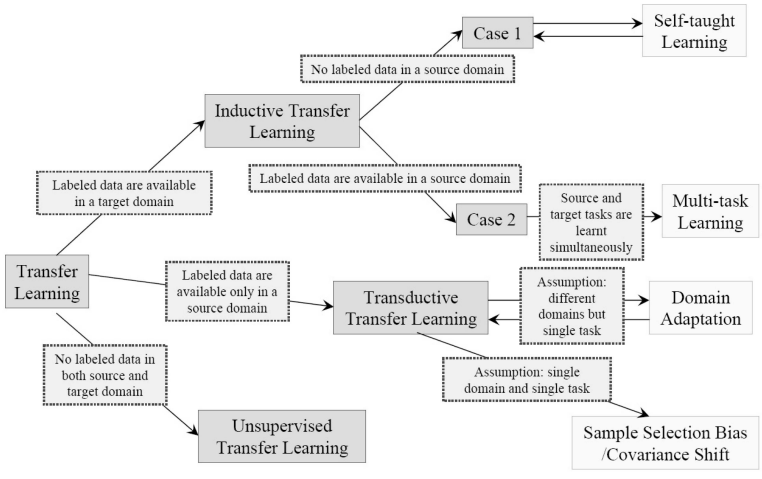
\includegraphics[width=350pt,height=200pt]{pictures/transfer_learning_types.PNG}
  \caption{Overview of the different types of transfer learning.\cite{pan2009survey}}
  \label{fig:transfer_learning_overview}
\end{figure} 
\subsubsection{Relevant Algorithms}
\subsection{Network generation process with PQ-Net++}



\section{Method}
\subsection{Suitable Algorithm and Adjustments}
\subsection{Whatever new Concept we propose}
\subsection{Architecture}
\subsection{Source and Target Objects}
\subsection{Data Generation}
\subsection{Important Aspects}

\section{Application of algorithms}

\section{Experiments}

\section{Implementation in a Bin Picking Cell}

\section{Conclusions}
\subsection{Discussions}
\subsection{Limitations}
\subsection{Future Scope}

\section{Summary}

\section*{List of Acronyms}
\addcontentsline{toc}{section}{List of Acronyms}

\begin{acronym}
    \acro{CNN}{Convolutional Neural Network}
    \acro{FCN}{Fully Connected Network}
    \acro{ReLU}{Rectified Linear Unit}
    \acro{ML}{Machine Learning}
    \acro{AI}{Artificial Intelligence}
    \acro{DBSCAN}{Density-Based Spatial Clustering of Applications with Noise}
    \acro{HDBSCAN}{Hierarchical Density-Based Spatial Clustering of Applications with Noise}
\end{acronym}
\addcontentsline{toc}{section}{List of Figures}
\listoffigures
\addcontentsline{toc}{section}{List of Tables}
\listoftables
\section*{List of Symbols}
\addcontentsline{toc}{section}{List of Symbols}


% \printunsrtglossary[type=symbols,style=long,title={List of Symbols}]


% =========================================================================
\printbibliography[heading=bibintoc,title={Bibliography}]
\end{document}
